\documentclass{beamer}


% Beamer settings
\usecolortheme{rose}
\beamertemplatenavigationsymbolsempty
\setbeamertemplate{footline}[frame number]

\titlegraphic{%

\includegraphics[height=1cm]{logo-full-colour.png}}

\addtobeamertemplate{frametitle}{}{%
\begin{tikzpicture}[remember picture,overlay]
\node[anchor=north east,yshift=2pt] at (current page.north east) {
\includegraphics[height=1cm]{logo-full-colour.png}};
\end{tikzpicture}}

% Packages
\usepackage{amsmath}

\usepackage{tikz}
\usetikzlibrary{positioning}
\usetikzlibrary{fit}

\usepackage{pgfplots}
\usepgfplotslibrary{fillbetween}

\usepackage{minted}
\usepackage[T1]{fontenc} % Required by minted to ensure dollar signs are produced instead of pound (sterling) signs

\usepackage{multicol}

\usepackage{booktabs}

\usepackage{adjustbox}

% Author
\author{Simon McIntosh-Smith \& Tom Deakin\\University of Bristol}

\date{}



\title{OpenMP Recap}
\subtitle{Advanced High Performance Computing}

\begin{document}

\frame{\titlepage}

%-------------------------------------------------------------------------------
\subsection{Compiler flags}
\begin{frame}[fragile]
\frametitle{Building with OpenMP}

Turn on OpenMP in the compiler:
\begin{minted}{bash}
gcc *.c -fopenmp   # GNU
icc *.c -qopenmp   # Intel
\end{minted}

To also use the API calls within the code, include the library header:
\begin{minted}{c}
#include <omp.h>
\end{minted}

\begin{alertblock}{Note}
No need to include the library if only using the compiler directives.
The library only gets you the API calls.
\end{alertblock}
\end{frame}

%-------------------------------------------------------------------------------
\section{Memory and execution model}
\begin{frame}
\frametitle{Shared memory}
OpenMP is for shared memory programming: all threads have access to a shared address space.

An HPC node consisting of two multi-core CPUs.
\begin{center}
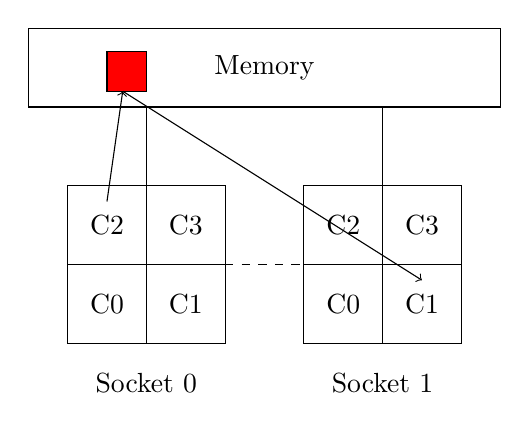
\begin{tikzpicture}
  % Draw 4 cores for socket 0
  \draw (0,0) rectangle (1,1);
  \draw (0.5,0.5) node {C0};
  \draw (1,0) rectangle (2,1);
  \draw (1.5,0.5) node {C1};
  \draw (0,1) rectangle (1,2);
  \draw (0.5,1.5) node {C2};
  \draw (1,1) rectangle (2,2);
  \draw (1.5,1.5) node {C3};
  \draw (1,-0.5) node {Socket 0};

  % Draw 4 cores for socket 1
  \draw (3,0) rectangle (4,1);
  \draw (3.5,0.5) node {C0};
  \draw (4,0) rectangle (5,1);
  \draw (4.5,0.5) node {C1};
  \draw (3,1) rectangle (4,2);
  \draw (3.5,1.5) node {C2};
  \draw (4,1) rectangle (5,2);
  \draw (4.5,1.5) node {C3};
  \draw (4,-0.5) node {Socket 1};

  % Draw large memory
  \draw (-0.5,3) rectangle (5.5,4);
  \draw (2.5,3.5) node {Memory};

  % Connect sockets to memory
  \draw (1,2) -- (1,3);
  \draw (4,2) -- (4,3);
  \draw[dashed] (2,1) -- (3,1); % QPI

  % Show memory shared
  \pause
  \draw[fill=red] (0.5,3.2) rectangle (1,3.7);
  \draw[->] (0.5,1.8) -- (0.7,3.2);
  \draw[->] (0.7,3.2) -- (4.5,0.8);

\end{tikzpicture}
\end{center}
\emph{All} threads (each running on a core) can access the same memory.

Different to MPI, where one process cannot see the memory of another without explicit communication.

\end{frame}

%-------------------------------------------------------------------------------
\begin{frame}
\frametitle{Fork-join model}
Serial/sequential execution:
\begin{center}
\begin{tikzpicture}
  \draw[->] (0,0) -- (8,0);
\end{tikzpicture}
\end{center}

\pause

In a \emph{fork-join} model, code starts serial, \emph{forks} a \emph{team} of threads then \emph{joins} them back to serial execution.
\begin{center}
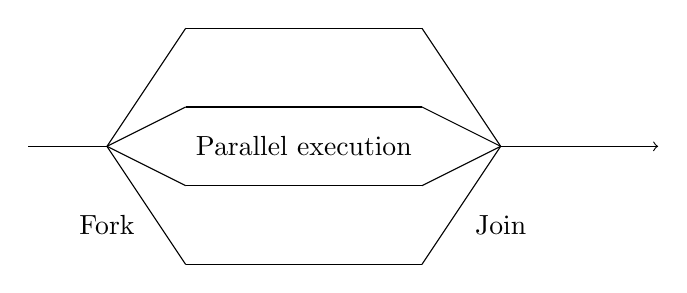
\begin{tikzpicture}
  \draw (0,0) -- (1,0);

  % Fork
  \draw (1,0) -- (2,1.5);
  \draw (1,0) -- (2,0.5);
  \draw (1,0) -- (2,-0.5);
  \draw (1,0) -- (2,-1.5);
  \draw (1,-1) node {Fork};

  % Run in parallel
  \draw (2,1.5)  -- (5,1.5);
  \draw (2,0.5)  -- (5,0.5);
  \draw (2,-0.5) -- (5,-0.5);
  \draw (2,-1.5) -- (5,-1.5);
  \draw (3.5,0) node {Parallel execution};

  % Join
  \draw (5,1.5)  -- (6,0);
  \draw (5,0.5)  -- (6,0);
  \draw (5,-0.5) -- (6,0);
  \draw (5,-1.5) -- (6,0);
  \draw (6,-1) node {Join};

  % Serial end
  \draw[->] (6,0) -- (8,0);
\end{tikzpicture}
\end{center}

Nested threads are allowed, where a thread forks its own team of threads. This is not often necessary, or even useful. However, OpenMP run-times are now clever at avoiding unnecessary thread creation/destruction, so the overhead of entering and leaving parallel regions may be negligible.
\end{frame}

%-------------------------------------------------------------------------------
\section{Going parallel}
\begin{frame}[fragile]
\frametitle{Creating OpenMP threads}
\begin{minted}[frame=single, linenos]{c}
int main(void) {

#pragma omp parallel
  printf("Hello\n");

}
\end{minted}

Threads \emph{redundantly} execute code in the block.

Every thread will output \mintinline{bash}|Hello|.

Threads are synchronised at the end of the parallel region.

Parallel region defined by structured block of code.

\end{frame}


%-------------------------------------------------------------------------------
\begin{frame}[fragile]
\frametitle{Setting number of threads}
The recommended approach is to let OpenMP set the number of threads for you at run-time. However, it is possible to set the number of threads to launch yourself. Useful for scaling tests etc.

OpenMP has 3 ways to do this:
\begin{itemize}
  \item Environment variables
  \begin{minted}{bash}
  OMP_NUM_THREADS=16
  \end{minted}

  \item API calls
  \begin{minted}{c}
  omp_set_num_threads(16);
  \end{minted}

  \item Clauses
  \begin{minted}{c}
  #pragma omp parallel num_threads(16)
  \end{minted}
\end{itemize}

In general it's better to use environment variables if you need to do this, as this approach gives you more flexibility at runtime.
\end{frame}

%-------------------------------------------------------------------------------
\begin{frame}[fragile]
\frametitle{Thread API calls}
Most parallel programs are written in a SPMD style: \newline
{\bf S}ingle {\bf P}rogram, {\bf M}ultiple {\bf D}ata.
\begin{itemize}
  \item Remember MPI has a SPMD model.
  \item Threads run the same code, and use their ID to work out which data to operate on.
  \item The SPMD approach requires lots of bookkeeping.
\end{itemize}

The OpenMP API gives you calls to determine thread information when \emph{inside} a parallel region:
\begin{itemize}
  \item Get number of threads
    \begin{minted}{c}
    nthreads = omp_get_num_threads();
    \end{minted}

  \item Get thread ID
    \begin{minted}{c}
    tid = omp_get_thread_num();
    \end{minted}

\end{itemize}
\end{frame}

%-------------------------------------------------------------------------------
\begin{frame}[fragile]
\frametitle{Vector add example}
Add parallel region around work, and use {\bf worksharing} constructs to distribute iterations across threads.
\begin{minted}[frame=single]{c}
  #pragma omp parallel for
  for (int i = 0; i < N; ++i) {
    c[i] = a[i] + b[i];
  }
\end{minted}
\begin{itemize}
  \item This starts a parallel region, forking a team of threads.
  \item Each thread then gets a portion of the iteration space and computes the loop body in parallel.
  \item Implicit synchronisation point at the end of loop.
  \item Threads finally join again; later code executes sequentially.
\end{itemize}

Much simpler than using the API calls to share the work (as you found out with the MPI assignment).
\end{frame}

%-------------------------------------------------------------------------------
\section{Scheduling}
\begin{frame}[fragile]
\frametitle{The Schedule clause}
\begin{itemize}
  \item The worksharing clauses use default rules for assigning loop iterations to threads.
  \item Can use the \mintinline{c}|schedule| clause to specify the distribution.
  \item General format:
    \begin{minted}{c}
      #pragma omp parallel for schedule(...)
    \end{minted}
\end{itemize}
The next slides go through the options, using the following loop as an example:
\begin{minted}[frame=single]{c}
#pragma omp parallel for num_threads(4)
for (int i = 0; i < 100; ++i) {
  ... // loop body
}
\end{minted}

\end{frame}

%-------------------------------------------------------------------------------
\begin{frame}[fragile]
\frametitle{Static schedule}
\begin{minted}{c}
schedule(static)
schedule(static,16)
\end{minted}

\begin{itemize}
\item Static schedule divides the iterations into chunks and assigns chunks to threads in a round-robin manner.
\item If no chunk size is specified (the default), the iteration space is divided roughly equally across the threads.
\end{itemize}
For our example loop:
\begin{columns}
\begin{column}{0.5\textwidth}
  \mintinline{fortran}|schedule(static)|
  \begin{tabular}{cc}
  \toprule
  Thread ID & Iterations \\
  \midrule
  0 &  0--24 \\
  1 & 25--49 \\
  2 & 50--74 \\
  3 & 75--99 \\
  \bottomrule
  \end{tabular}
\end{column}

\begin{column}{0.5\textwidth}
  \mintinline{fortran}|schedule(static,16)|
  \begin{tabular}{cc}
  \toprule
  Thread ID & Iterations \\
  \midrule
  0 &  0--15, 64--79 \\
  1 & 16--31, 80--95 \\
  2 & 32--47, 96--99 \\
  3 & 48--63 \\
  \bottomrule
  \end{tabular}
\end{column}
\end{columns}

\end{frame}

%-------------------------------------------------------------------------------
\begin{frame}[fragile]
\frametitle{Dynamic schedule}
\begin{minted}{c}
schedule(dynamic)
schedule(dynamic,16)
\end{minted}

\begin{itemize}
  \item Iteration space is divided into chunks according to chunk size.
  \item If no chunk size specified, default size is one.
  \item Each thread requests and executes a chunk, until no more chunks remain.
  \item Useful for unbalanced work-loads if some threads complete work (a lot) faster than others.
\end{itemize}

For our example with a chunk size of 16:
\begin{itemize}
  \item The iteration space is split into chunks of 16 (the last chunk may be smaller).
  \item Each threads gets one chunk, then requests a new chunk to work on.
\end{itemize}

\end{frame}

%-------------------------------------------------------------------------------
\begin{frame}[fragile]
\frametitle{Guided schedule}
\begin{minted}{c}
schedule(guided)
schedule(guided,16)
\end{minted}

\begin{itemize}
  \item Similar to dynamic, except the chunk size decreases over time.
  \item The granularity of work chunks gets finer over time.
  \item If no chunk size is specified, the default size is one.
  \item Useful to try to mitigate overheads of a \mintinline{c}|dynamic| schedule by starting with large chunks of work.
\end{itemize}

For our example with a chunk size of 16:
\begin{itemize}
  \item Each thread gets a chunk of 16 to work on.
  \item Each thread requests a new chunk, which might be smaller than 16.
\end{itemize}

\end{frame}

%-------------------------------------------------------------------------------
\begin{frame}[fragile]
\frametitle{Other schedules}
\begin{minted}{c}
schedule(auto)
\end{minted}
\begin{itemize}
  \item Let the compiler or runtime choose the schedule.
\end{itemize}

\vfill

\begin{minted}{c}
schedule(runtime)
\end{minted}
\begin{itemize}
  \item Get the schedule from the \mintinline{bash}|OMP_SCHEDULE| environment variable.
\end{itemize}

\begin{block}{Recommendation}
Use a \mintinline{c}|static| schedule unless there is a good reason not to!
\mintinline{c}|static| is usually the fastest of all the options.
The choice of schedule is an advanced tuning option.
\end{block}

\end{frame}

%-------------------------------------------------------------------------------
\section{Synchronisation}
\begin{frame}[fragile]
\frametitle{The nowait clause}
\begin{itemize}
  \item Consider a series of independent loops.
  \item Threads must wait/synchronise at the end of the loop.
  \item But it might be possible to amortise multiple synchronisations using the \mintinline{c}|nowait| clause.
  \item When a thread finishes the first loop, it starts on the next loop.
\end{itemize}

\begin{minted}[fontsize=\small, linenos, frame=single]{c}
#pragma omp parallel
{
  #pragma omp for nowait
  for (int i = 0; i < N; ++i) {
    A[i] = i;
  } // no barrier

  #pragma omp for
  for (int i = 0; i < N; ++i) {
    B[i] = i;
  }       // Implicit barrier
} // Implicit barrier
\end{minted}
\end{frame}

%-------------------------------------------------------------------------------

\section{Data sharing}
\begin{frame}
\frametitle{Data sharing}
Remember: OpenMP is a \emph{shared memory} programming model.
\begin{itemize}
  \item By default, all data is available to all threads.
  \item There is a single copy of \emph{shared} data.
\end{itemize}

\vfill

You must specify which data should be \emph{private} to each thread.
\begin{itemize}
  \item Each thread then has local (stack) space for each private variable.
  \item Each copy is only visible to its associated thread.
\end{itemize}

\end{frame}


%-------------------------------------------------------------------------------
\begin{frame}
\frametitle{Variables on the heap}
\begin{itemize}
  \item All data on the heap is shared.
  \item Therefore all the data from \mintinline{c}|malloc| is shared.
  \item You must ensure that different threads do not write to the same element of these arrays.
\end{itemize}

\begin{alertblock}{Caution}
Setting a data sharing clause on a heap variable only effects the metadata of the variable.
The pointer could be private, but the target data will still be shared.
\textit{This is a common source of bugs.}
\end{alertblock}
\end{frame}

%-------------------------------------------------------------------------------
\section{Data clauses}
\begin{frame}
\frametitle{Data clauses}
\begin{itemize}
  \item \mintinline{c}|shared(x)|
    There is one copy of the \mintinline{c}|x| variable. The programmer must ensure synchronisation.
  \item \mintinline{c}|private(x)|
    Each thread gets its own local \mintinline{c}|x| variable. It is not initialised. The value of the original \mintinline{c}|x| variable is undefined on region exit.
  \item \mintinline{c}|firstprivate(x)|
    Each thread gets its own \mintinline{c}|x| variable, and it is initialised to the value of the original variable entering the region.
  \item \mintinline{c}|lastprivate(x)|
    Used for loops. Each thread gets its own \mintinline{c}|x| variable, and on exiting the region the original variable is updated taking the value from the sequentially last iteration.
\end{itemize}

These are the most common clauses that are needed.
\end{frame}

%-------------------------------------------------------------------------------
\subsection{Private example}
\begin{frame}[fragile]
\frametitle{Private example}
Simple \mintinline{c}|for| loop, which sets a variable to the iteration number.
Each iteration prints out the current and next value of \mintinline{c}|x|, along with the thread number.
We will explore what happens with different data sharing clauses.

\begin{minted}[linenos,breaklines,frame=single, fontsize=\small]{c}
  int x = -1;
  #pragma omp parallel for private(x) / firstprivate(x) / lastprivate(x)
  for (int i = 0; i < N; ++i) {
    printf("Thread %d setting x=%d to %d\n", omp_get_thread_num(), x, i);
    x = i;
  }
\end{minted}
N is set to 10.
Run using 4 threads.
\end{frame}

%-------------------------------------------------------------------------------
\begin{frame}[fragile]
\frametitle{Private example}
\begin{minted}{bash}
private:
 before: x=-1
  Thread 1 setting x=0 to 3
  Thread 2 setting x=0 to 6
  Thread 3 setting x=0 to 8
  Thread 0 setting x=0 to 0
  Thread 1 setting x=3 to 4
  Thread 2 setting x=6 to 7
  Thread 3 setting x=8 to 9
  Thread 0 setting x=0 to 1
  Thread 1 setting x=4 to 5
  Thread 0 setting x=1 to 2
 after: x=-1
\end{minted}
Each thread starts with its own \mintinline{c}|x|.
No guarantees of initial value, but happened to be zero this time.
\end{frame}

%-------------------------------------------------------------------------------
\begin{frame}[fragile]
\frametitle{Firstprivate example}
\begin{minted}{bash}
firstprivate:
 before: x=-1
  Thread 3 setting x=-1 to 8
  Thread 2 setting x=-1 to 6
  Thread 1 setting x=-1 to 3
  Thread 0 setting x=-1 to 0
  Thread 3 setting x=8 to 9
  Thread 2 setting x=6 to 7
  Thread 1 setting x=3 to 4
  Thread 0 setting x=0 to 1
  Thread 1 setting x=4 to 5
  Thread 0 setting x=1 to 2
 after: x=-1
\end{minted}
Each thread starts with its own \mintinline{c}|x|, which set to the value of \mintinline{c}|x| before entering the \mintinline{c}|parallel| region, -1.
\end{frame}

%-------------------------------------------------------------------------------
\begin{frame}[fragile]
\frametitle{Lastprivate example}
\begin{minted}{bash}
lastprivate:
 before: x=-1
  Thread 3 setting x=2 to 8
  Thread 2 setting x=1 to 6
  Thread 1 setting x=0 to 3
  Thread 3 setting x=8 to 9
  Thread 0 setting x=-1 to 0
  Thread 2 setting x=5 to 7
  Thread 1 setting x=3 to 4
  Thread 0 setting x=0 to 1
  Thread 1 setting x=4 to 5
  Thread 0 setting x=1 to 2
 after: x=10
\end{minted}
Each thread starts with its own \mintinline{c}|x|, which set to to a garbage value.
On exiting the region, the original \mintinline{c}|x| is set to the value of the last iteration of the loop, 10.
\end{frame}

%-------------------------------------------------------------------------------
\section{Default data sharing}
\begin{frame}
\frametitle{Choosing default data sharing}

\begin{itemize}
  \item You can force yourself to specify everything manually by using the \mintinline{c}|default(none)| attribute.
  \item This is good practice, as it avoids lots of bugs commonly introduced when you get this wrong. 
  \item Using \mintinline{c}|default(none)| also makes you think about how you're using each of your data structures (a good thing).
\end{itemize}

\end{frame}

%-------------------------------------------------------------------------------
\section{Reductions}
\begin{frame}[fragile]
\frametitle{Reductions}
Loops often have a reduction operation: a value from each iteration is combined into a single value.
To do this in parallel in OpenMP, use the \mintinline{c}|reduction| clause on a worksharing loop.
Specify the operation and the variable.
\begin{multicols}{2}
\begin{itemize}
  \item \mintinline{c}|reduction(+:var)|
  \item \mintinline{c}|reduction(-:var)|
  \item \mintinline{c}|reduction(*:var)|
  \item \mintinline{c}|reduction(&:var)|
  \item \begin{minted}{c}
reduction(|:var)
  \end{minted}
  \item \mintinline{c}|reduction(^:var)|
  \item \mintinline{c}|reduction(&&:var)|
  \item \begin{minted}{c}
reduction(||:var)
  \end{minted}
  \item \mintinline{c}|reduction(max:var)|
  \item \mintinline{c}|reduction(min:var)|
\end{itemize}
\end{multicols}

Can also do array reductions. Each element of the array is treated as its own, separate, reduction.
Similar to:
\begin{minted}[breaklines]{fortran}
MPI_Allreduce(MPI_IN_PLACE, arr, N, MPI_DOUBLE, MPI_SUM, 0, MPI_COMM_WORLD, ierr)
\end{minted}

\end{frame}

%-------------------------------------------------------------------------------
\begin{frame}[fragile]
\frametitle{Pi reduction}
Much simpler to write using the \mintinline{c}|reduction| clause ---  needs a single directive:
\begin{minted}[linenos,breaklines,frame=single]{c}
  sum = 0.0;
  step = 1.0/num_steps;
  #pragma omp parallel for private(x) reduction(+:sum)
  for (int i = 1; i <= num_steps; ++i) {
    x = (i-0.5)*step;
    sum = sum + (4.0/(1.0+x*x));
  }
  pi = step * sum;
\end{minted}

\end{frame}

%-------------------------------------------------------------------------------

\section{NUMA}
\begin{frame}
\frametitle{NUMA Architecture}

Recall this cartoon of a dual-socket, shared memory system:
\begin{center}
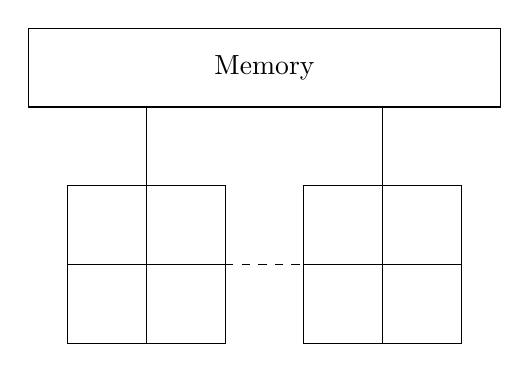
\begin{tikzpicture}
  % Draw 4 cores for socket 0
  \draw (0,0) rectangle (1,1);
  \draw (1,0) rectangle (2,1);
  \draw (0,1) rectangle (1,2);
  \draw (1,1) rectangle (2,2);

  % Draw 4 cores for socket 1
  \draw (3,0) rectangle (4,1);
  \draw (4,0) rectangle (5,1);
  \draw (3,1) rectangle (4,2);
  \draw (4,1) rectangle (5,2);

  % Draw large memory
  \draw (-0.5,3) rectangle (5.5,4);
  \draw (2.5,3.5) node {Memory};

  % Connect sockets to memory
  \draw (1,2) -- (1,3);
  \draw (4,2) -- (4,3);
  \draw[dashed] (2,1) -- (3,1); % QPI

\end{tikzpicture}
\end{center}

\emph{All} threads (each running on a core) can access all the memory in the node.

\end{frame}
%-------------------------------------------------------------------------------

\begin{frame}
\frametitle{NUMA Architecture}
\begin{itemize}
  \item In reality on a dual-socket system each \emph{socket} is physically connected to half of the memory.
  \item Still shared memory: all cores can access all the memory.
  \item A core in the first socket wanting memory attached to the other socket must:
    \begin{itemize}
      \item Go via the socket-to-socket interconnect.
      \item Access memory via the other socket's memory controllers.
    \end{itemize}
  \item Accessing memory from other socket is slower than access from own socket.
\end{itemize}
\begin{center}
\resizebox{!}{3.5cm}{
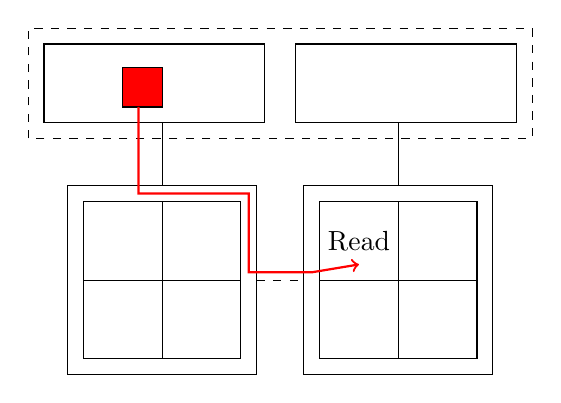
\begin{tikzpicture}
  % Draw 4 cores for socket 0
  \foreach \i in {0,1,3,4} {
    \foreach \j in {0, 1} {
      \draw (\i,\j) rectangle (\i+1,\j+1);
    }
  }

  % Draw sockets around cores
  \draw (-0.2, -0.2) rectangle (2.2, 2.2);
  \draw (2.8, -0.2) rectangle (5.2, 2.2);

  % Draw large memory
  \draw (-0.5,3) rectangle (2.3,4);
  \draw (2.7,3) rectangle (5.5,4);
  \draw[dashed] (-0.7,2.8) rectangle (5.7,4.2);

  % Connect sockets to memory
  \draw (1,2.2) -- (1,3);
  \draw (4,2.2) -- (4,3);
  \draw[dashed] (2.2,1) -- (2.8,1); % QPI

  % Show memory shared
  \pause
  \draw[fill=red] (0.5,3.2) rectangle (1,3.7);
  \draw (3.5,1.5) node {Read};
  \pause
  \draw[->,red,thick] (0.7,3.2) -- (0.7,2.1) -- (2.1,2.1) -- (2.1,1.1) -- (2.9,1.1) -- (3.5,1.2);

\end{tikzpicture}
}
\end{center}
\end{frame}

%-------------------------------------------------------------------------------

\subsection{NUMA on BCp4}
\begin{frame}[fragile]
\frametitle{NUMA on BCp4}
You can discover the NUMA configuration of any Linux node with \mintinline{bash}|numactl --hardware|.


\begin{minted}[fontsize=\footnotesize,frame=single]{shell-session}
[cssnmis@bc4login2 ~]$ numactl --hardware
available: 2 nodes (0-1)
node 0 cpus: 0 1 2 3 4 5 6 7 8 9 10 11 12 13
node 0 size: 130237 MB
node 0 free: 54862 MB
node 1 cpus: 14 15 16 17 18 19 20 21 22 23 24 25 26 27
node 1 size: 131072 MB
node 1 free: 123735 MB
node distances:
node   0   1 
  0:  10  21 
  1:  21  10 
\end{minted}

\end{frame}



%-------------------------------------------------------------------------------
\begin{frame}
\frametitle{Memory allocation}
\begin{itemize}
  \item What happens when you run \mintinline{c}|A = malloc(sizeof(double) * N);|?
  \pause
  \item Allocating memory does not necessarily allocate memory!
  \item Memory is allocated when it's first used (i.e. \mintinline{c}|A[i] = 1.0;|), one \emph{page} at a time.
  \item OS tends to use a \emph{first touch policy}.
  \item Memory is allocated in the closest NUMA region to the thread that first touches the data (page by page).
  \item Ideally want threads to use data in local NUMA region to reduce socket-to-socket interconnect transfers.
\end{itemize}
\end{frame}

%-------------------------------------------------------------------------------


\subsection{First touch}
\begin{frame}[fragile]
\frametitle{Taking advantage of first touch}
Parallelising your data initialisation routine might mean your main loops go faster!


%\begin{minted}[fontsize=\footnotesize,linenos,frame=single]{c}
\begin{minted}[linenos,breaklines,frame=single,fontsize=\scriptsize]{c}
// Allocate and initialise vectors
double *A = malloc(sizeof(double) * N);
double *B = malloc(sizeof(double) * N);
double *C = malloc(sizeof(double) * N);

// Arrays A, B and C all initialised serially, by core 0 in NUMA region 0

for (int i = 0; i < N; ++i) {
  A[i] = 1.0;
  B[i] = 2.0;
  C[i] = 0.0;
}

// Vector add
#pragma omp parallel for
for (int i = 0; i < N; ++i) {
  C[i] = A[i] + B[i];
}
\end{minted}

\end{frame}

\subsection{First touch}
\begin{frame}[fragile]
\frametitle{Taking advantage of first touch}
Parallelising your data initialisation routine might mean your main loops go faster!


%\begin{minted}[fontsize=\footnotesize,linenos,frame=single]{c}
\begin{minted}[linenos,breaklines,frame=single,fontsize=\scriptsize]{c}
// Allocate and initialise vectors
double *A = malloc(sizeof(double) * N);
double *B = malloc(sizeof(double) * N);
double *C = malloc(sizeof(double) * N);

// Arrays A, B and C all initialised in parallel, ending up spread across the NUMA regions
#pragma omp parallel for
for (int i = 0; i < N; ++i) {
  A[i] = 1.0;
  B[i] = 2.0;
  C[i] = 0.0;
}

// Vector add
#pragma omp parallel for
for (int i = 0; i < N; ++i) {
  C[i] = A[i] + B[i];
}
\end{minted}

\end{frame}

%-------------------------------------------------------------------------------
\begin{frame}
\frametitle{NUMA-aware}
\begin{itemize}
  \item Parallelise your initialisation routines the same way you parallelise the main loops.
  \item This will ensure that each thread touches the same data in initialisation and compute.
  \item Should reduce the number of remote memory accesses needed, improving run times and reducing variability.
  \item But, the OS is allowed to move threads from one core to another, and even between sockets.
  \item This could mess up your NUMA aware code!
\end{itemize}
\end{frame}

%-------------------------------------------------------------------------------
\section{Thread affinity}
\begin{frame}
\frametitle{Pinning threads}
\begin{itemize}
  \item OpenMP gives you the controls to pin threads to specific cores.
  \item Exposed as \emph{places} and \emph{thread pinning policy} to those places.
  \item By default there is one place consisting of all the cores.
  \item Use the \mintinline{bash}|OMP_PROC_BIND| environment variable to set pinning for all \mintinline{c}|parallel| regions.
  \item Can use the \mintinline{bash}|proc_bind| clause for control of specific regions, but we advise against this.
\end{itemize}
\end{frame}

%-------------------------------------------------------------------------------
\begin{frame}
\frametitle{OMP\_PROC\_BIND}
\begin{itemize}
  \item \mintinline{bash}|OMP_PROC_BIND=false|: Often the default; threads may move! \mintinline{fortran}|proc_bind| clauses ignored.
  \item \mintinline{bash}|OMP_PROC_BIND=true|: Threads won't move, and follow \mintinline{fortran}|proc_bind| clauses or else the implementation default pinning.
  \item \mintinline{bash}|OMP_PROC_BIND=master|: Threads pinned to same place as master thread.
  \item \mintinline{bash}|OMP_PROC_BIND=close|: Threads are assigned to places close to the master thread.
  If \mintinline{bash}|OMP_NUM_THREADS==ncores|: thread 0 will pin to core 0; thread 1 will pin to core 1; etc
  \item \mintinline{bash}|OMP_PROC_BIND=spread|: Threads are assigned to places ``sparsely''.
  If \mintinline{bash}|OMP_NUM_THREADS==ncores|: thread 0 will pin to socket 0 core 0; thread 1 will pin to socket 1 core 0; thread 2 will pin to socket 0 core 1; etc.
\end{itemize}
\end{frame}

%-------------------------------------------------------------------------------
\begin{frame}
\frametitle{Places}
\begin{itemize}
  \item The affinity (policy) defines how threads are assigned to places.
  \item Places allow you to divide up the hardware resource, so that threads can be assigned to them.
  \item Default: one place with all cores.
  \item Use \mintinline{bash}|OMP_PLACES| environment variable to control.
  \item \mintinline{bash}|OMP_PLACES=thread|: each place is a single hardware thread.
  \item \mintinline{bash}|OMP_PLACES=cores|: each place is a single core (containing one or more hardware threads).
  \item \mintinline{bash}|OMP_PLACES=sockets|: each place contains the cores of a single socket.
  \item Can also use list notation: \mintinline{bash}|OMP_PLACES="{0:4},{4:4},{8:4},{12:4}"|
\end{itemize}
\end{frame}

%-------------------------------------------------------------------------------
\begin{frame}
\frametitle{Thread pinning summary}
\begin{itemize}
  \item In general, going to want to use \mintinline{bash}|OMP_PROC_BIND=true|.
  \item Sometimes \mintinline{bash}|spread| or \mintinline{bash}|close| gets better performance.
  \item Pinning rules can get complicated when there are multiple places, so prefer to use the predefined values.
  \item Most effective with a NUMA-aware implementation.
  \item Also helps reduce run-to-run timing variability.
  \item But must be careful with MPI+OpenMP pinning\dots
\end{itemize}
\end{frame}

%-------------------------------------------------------------------------------

\begin{frame}
\frametitle{Further reading}
\begin{itemize}
  \item NUMA: \url{https://www.thegeekdiary.com/what-is-numa-and-how-does-it-work-in-linux/}
  \item Linux first touch: \url{https://www.kernel.org/doc/html/v4.18/vm/numa.html?highlight=numa}
  \item Page migration: \url{https://www.kernel.org/doc/html/v4.18/vm/page_migration.html}
\end{itemize}


\end{frame}


%-------------------------------------------------------------------------------
\begin{frame}
\frametitle{Hints on serial optimisations}
\begin{itemize}
  \item Compiler optimisation (-Ofast et al)
  \item Simplify the expressions being calculated (help the compiler)
  \item Loop fusion (merge multiple passes over the grid into one)
  \item Remove redundant copy from \mintinline{C}|tmp_cell[]| to \mintinline{C}|cells[]| (pointer swap)
\end{itemize}
Once you have all those working
\begin{itemize}
  \item Vectorisation (may need AoS to SoA transformation)
%  \item Results in about another 2.5X, e.g. 22s $\rightarrow$ 8s for 128x128
\end{itemize}

\end{frame}

%-------------------------------------------------------------------------------



\end{document}
